\section{\label{sec:aufbau}Aufbau und Durchführung}
\subsection{Autokorrelation}
Im ersten Teil des Experiments werden die aus einem Strahlteiler ausgekoppelten Femtosekunden-Laserpulse 
charakterisiert. Da diese Laserpulse zu kurz sind, um sie mit herkömmlichen Methoden zu untersuchen, 
nutzen wir die Autokorrelation. Dabei wird der Puls durch sich selbst abgetastet. \\
Für den Aufbau des Michelson-Interferometers verwenden wir zunächst einen Justagelaser mit einer 
sichtbaren Wellenlänge. Dies vereinfacht die Überprüfung der räumlichen Überlagerung der Teilstrahlen. 
Abbildung~\ref{fig:autokorr} zeigt den schematischen Aufbau des Autokorrelators sowie die tatsächliche Umsetzung.
\begin{figure}[h!]
    \centering
    \subfloat[\centering Skizze des Aufbaus]{{\includegraphics[width=0.53\textwidth]{AutokorSkizze.png} }}
    \qquad
    \subfloat[\centering Realisierung]{{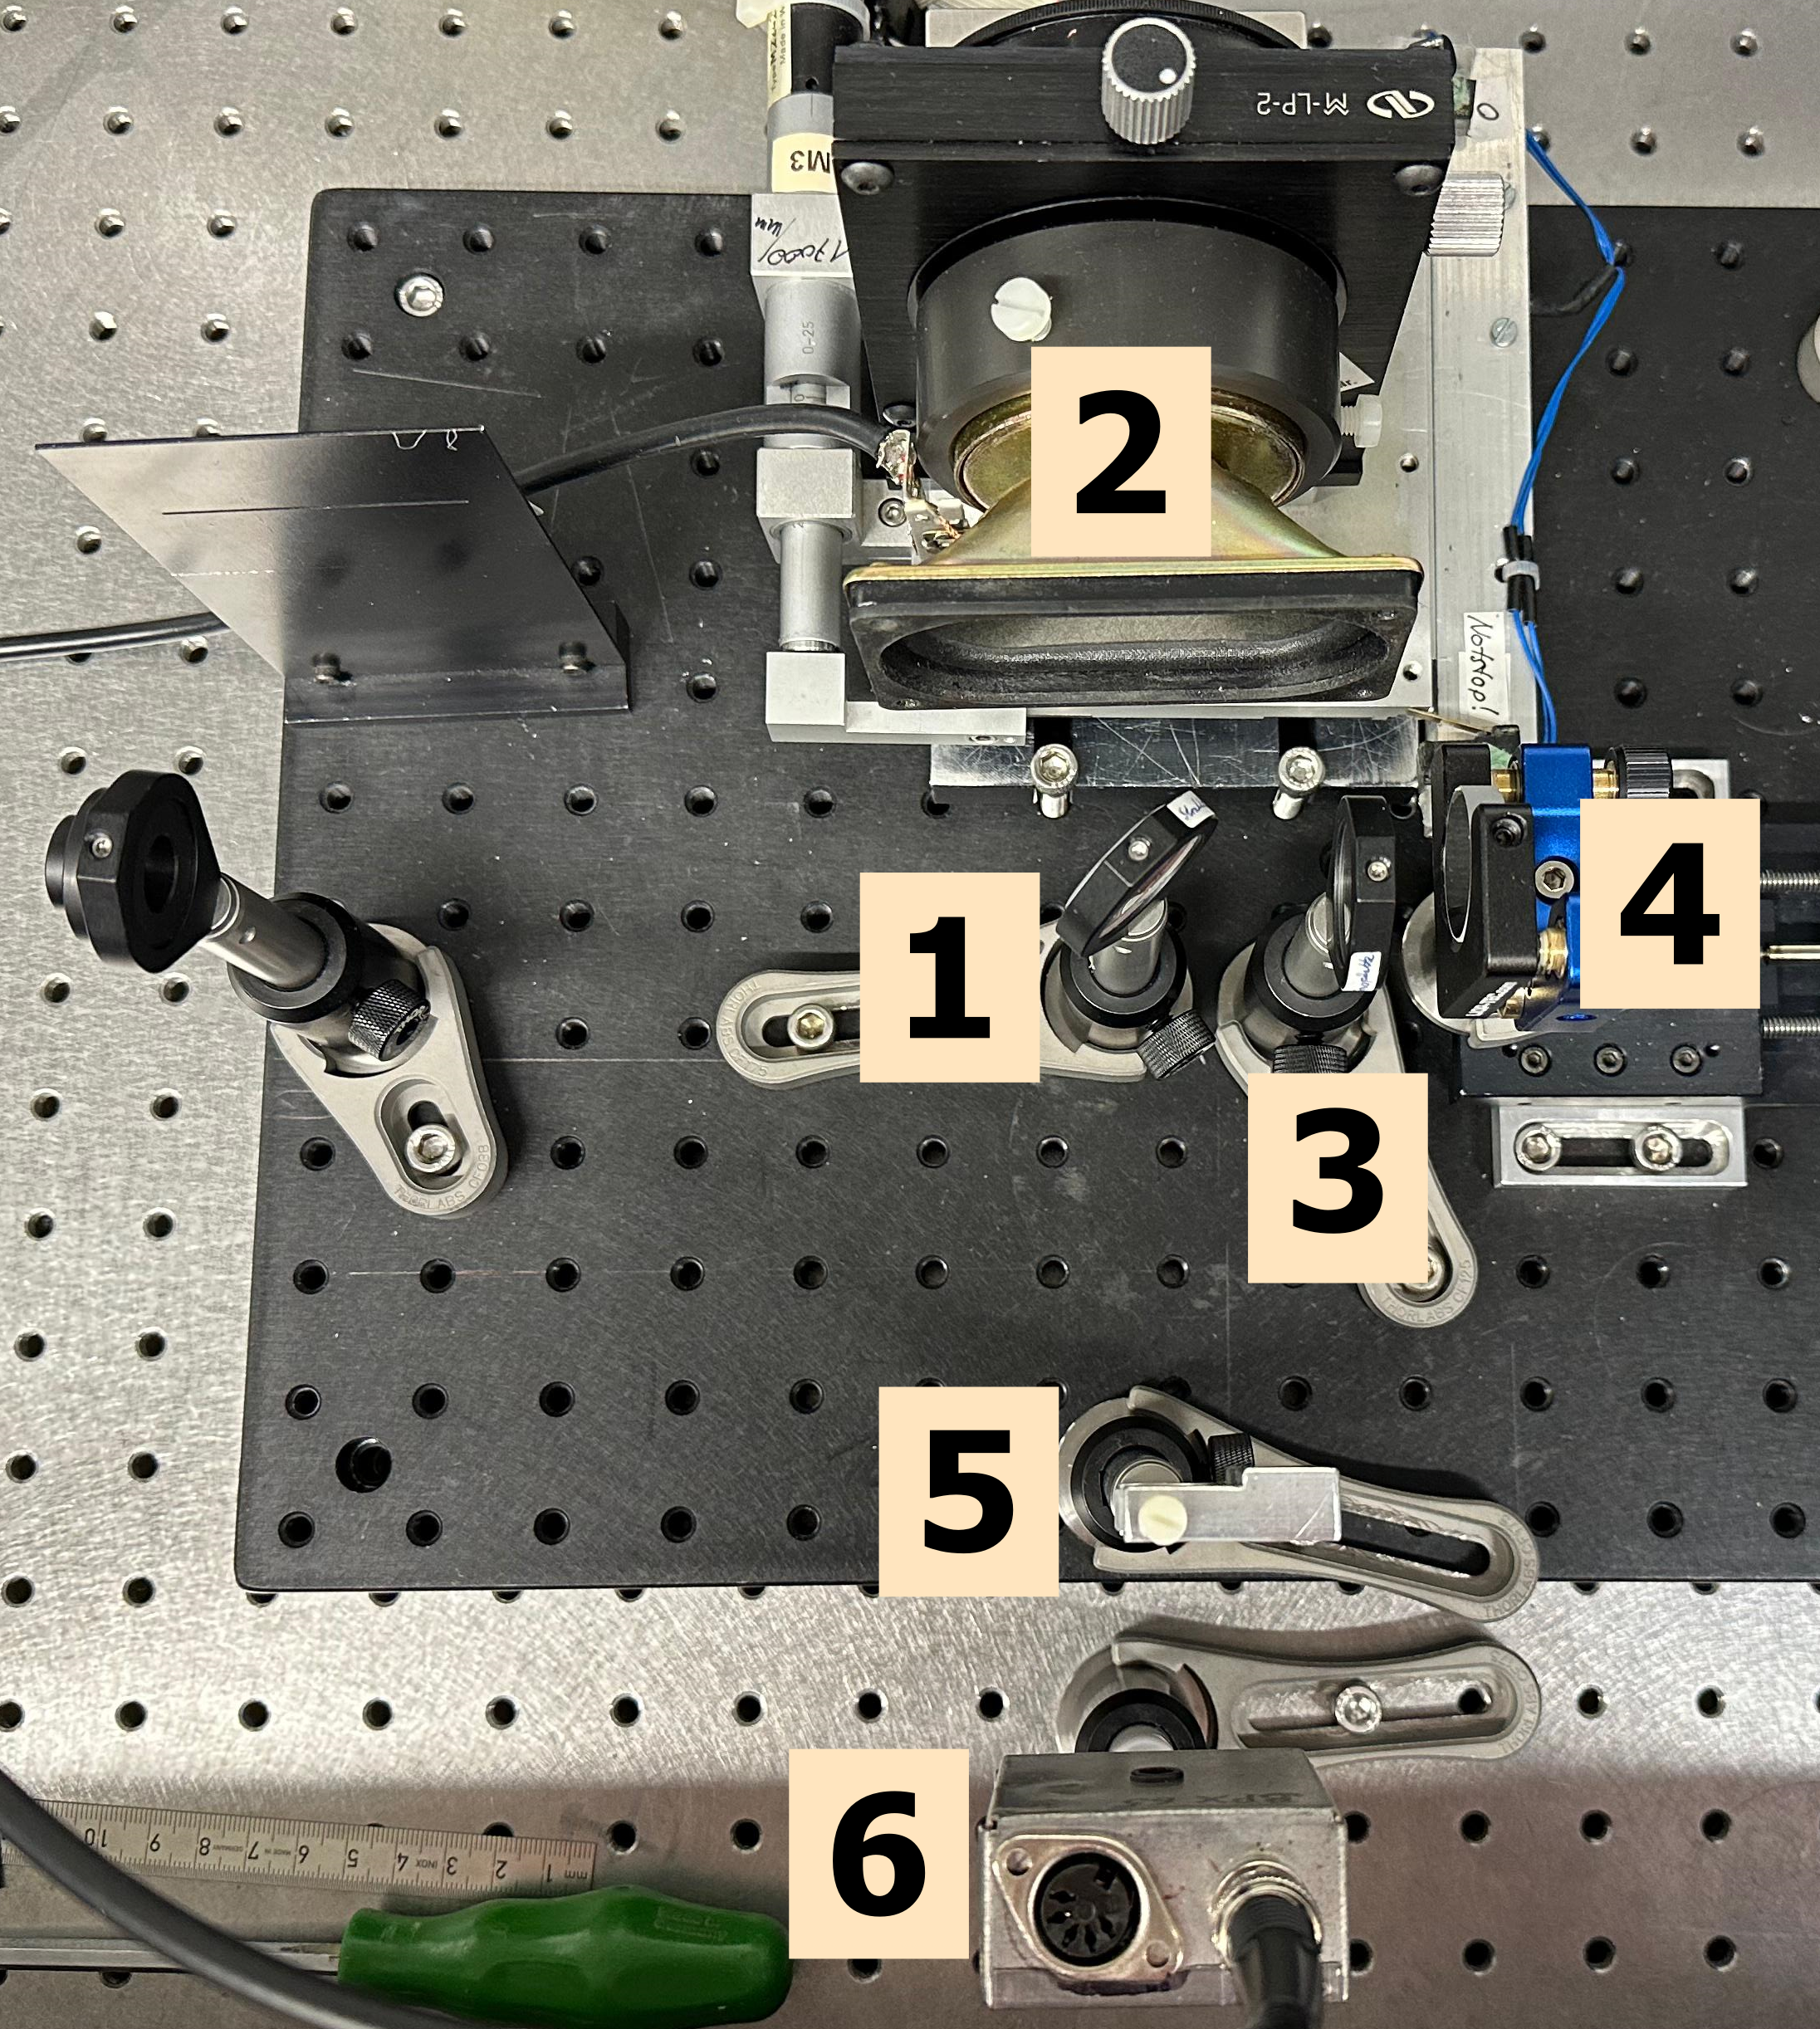
\includegraphics[width=0.39\textwidth]{Autokor.png} }}
    \caption{\label{fig:autokorr}a) Prinzipieller Aufbau eines Autokorrelators inkl.~Strahlengang und angedeuteter Pulsüberlagerung
    vor der Diode. Die Skizze wurde aus der Versuchsanleitung \cite{Anleitung} übernommen. \\
    b) Realisierter Aufbau: Von links trifft der Laserpuls in das Interferometer und wird am 50:50 Strahlteiler (1) aufgeteilt. 
    Am Lautsprecher (2), der auf einer Verschiebebühne platziert ist, ist ein Spiegel befestigt. Der andere Teilstrahl durchläuft die 
    Kompensationsplatte (3) bis zum Spiegel (4). Vor der Zwei-Photonen-Diode (6) wird 
    eine Sammellinse (5) platziert, um die Intensität zu bündeln und auf den Diodenchip zu fokussieren. \\
    Theoretischer und realisierter Aufbau unterscheiden sich in der Platzierung der Kompensationsplatte, was 
    auf die Orientierung des Strahlenteilers zurückzuführen ist, dessen Reflexschicht sich auf der zur 
    Kompensationsplatte zugewandten Seite befindet.}
\end{figure}\FloatBarrier \,\\
Der Lautsprecher wird mittels eines Funktionsgenerators angesteuert, der die Lautsprechermembran, 
an der der Spiegel befestigt ist, in Schwingungen versetzt. 
Dadurch wird die Weglänge eines der Teilstrahlen variabel, was zu einer zeitlichen Verzögerung 
$\Delta\tau$ zwischen beiden Teilpulsen führt. 
Nach der korrekten Justage der optischen Instrumente, überlagern sich die Strahlen räumlich und sind 
auf den Chip der Zwei-Photonen-Diode fokussiert. 
Diese registriert nur ein Signal, wenn zwei Photonen gleichzeitig absorbiert werden, 
was es ermöglicht, die Intensitätsautokorrelation $A^{(2)}(\Delta\tau)$ zu messen. Hierbei gilt
\begin{equation}
    A^{(2)}(\Delta\tau) = \int_{-\infty}^{\infty}\,dt\,I(t)I(t-\Delta\tau) = \int_{-\infty}^{\infty}\,dt\,\left\vert E(t) + E(t-\Delta\tau) \right\vert^{4}.
\end{equation}  
Für die Bestimmung des Laserpulses ist ein nichtlinearer Prozess erforderlich, da die lineare 
Autokorrelation gemäß dem Wiener-Chintschin-Theorem dieselben Informationen wie das Intensitätsspektrum enthält \cite{Anleitung}. 
Aus diesem Spektrum kann im Allgemeinen keine spezifische Pulsinformation extrahiert werden. \\
Das auf der Diode registrierte Signal setzt sich aus einem durchschnittlichen Hintergrundsignal, 
schnell oszillierenden interferometrischen Komponenten und einem relevanten Term, der von $\Delta\tau$ abhängt, 
zusammen (siehe Gl.~(2.6) in Ref.~\cite{Anleitung}). 
Nach der Justierung wird der Femtosekunden-Laser eingeschaltet, und mithilfe des Oszilloskops, 
das mit der Diode verbunden ist, wird die räumliche Überlagerung der Strahlen überprüft. 
Durch das Blockieren des Strahls kann die Stärke des Hintergrundsignals ermittelt werden, 
was Rückschlüsse auf die Qualität der räumlichen Überlagerung zulässt. 
Nachdem dieses Signal durch präzise Anpassung der optischen Instrumente maximiert wurde, 
wird einer der Spiegel mechanisch verschoben, bis eine zeitliche Überlagerung der geteilten Laserpulse 
erreicht ist. 
Die auf dem Oszilloskop angezeigte Intensitätsautokorrelationsfunktion wird daraufhin gespeichert, 
womit dieser Teil des Experiments erfolgreich abgeschlossen ist.\\

\subsection{Terahertz time-domain spectroscopy (THz-TDS)}
